\newpage
\thispagestyle{empty}
\chapter{Preliminaries}
In this chapter we present the basic theoretical knowledge necessary to understand this thesis. We begin by introducing graph theory, random walks and quantum walks. We then discuss the quantum search problem firstly introduced by Grover and the quantum walks implementation for the unstructured search by Childs and Goldstone. Then we present the adiabatic theorem and its application for computation with adiabatic evolution. Lastly we look at the differences between the quantum walks approach and the adiabatic evolution approach by Ronald and Cerf, which constitutes the basis from which our work is carried on.

\section{Introduction to graph theory}
A graph G is defined as a ordered pair $(V,E)$, where V is a set of vertices and E is a set of edges, which represent the connection between any two pair of vertices. A vertex is usually indicated by the coursive letter $v$, and the corresponding edge connecting $v$ to $w$ is given by $(v,w)$. \\

\noindent
A graph can be characterized by many properties. Throughout our work we will only consider \textit{simple graphs} characterized by being \textit{undirected}, namely the edges $E$ are symmetric, having no self loops such that $(v,v)\notin G$ and having no multiple equivalent edges. Additionally we require the graph to be \textit{connected}, where each vertex can be reached by any other, following a path through the available edges.

\noindent
It is then interesting to define the \textit{vertex degree} $d_j$, that represents, given a vertex $j$, the number of edges that are incident to the vertex $j$ (in the case of an undirected graph the degree does not dependend on the edges incident from or to the selected vertex). \\

\noindent
If indeed any two vertices $(i,j)$ are connected by an edge we define them as \textit{adjacent}, and from this we can construct an analytical representation of a graph, given by an N-dimensional square matrix called \textit{adjacency matrix}, usually referred as A. The adjacency matrix is defined as following \footnote{If we had to define the adjacency matrix for a general graph the value of $A_{ij}$ is not necessarily equal to one, but a general $a_{ij}$ since it takes into account the possibilities of self loops and multiple equivalent edges. For the simple graphs consider in this thesis the given definition suffices.}:
\begin{equation}
A_{ij} = \begin{cases} 1 & \mbox{if }(i,j)\in G \\ 0 & \mbox{otherwise} \end{cases}
\end{equation}
which represents the connectivity of the graph. \\
Furthermore, we can introduce a diagonal matrix $D$ that encodes the informations of the vertex degrees for a particular graph $G$. Calling the N vertices of the graph as $j=1,2..N$ the matrix D is defined as:
\begin{equation}
    D = diag(d_1,..., d_N)
\end{equation}
where $d_j$ is the degree of the vertex $j$.
In this particular context a natural operative basis arises, in which one can associate to each ordered vertex of the graph a vector of the standard basis of the N-dimensional vector space. \\ \\


In order to study the dynamics of the system we introduce a the \textit{Laplacian matrix L}, also known as the \textit{discrete Laplacian operator}. It is defined as
\begin{equation}
    L = D-A
\end{equation}
where $D$ is the diagonal degrees matrix and $A$ is the adjacenty matrix. The discrete Laplacian operator is the analog of the continous Laplace operator on discrete domain, and for the finite, undirected, simple and connected graphs that we're going to consider throughout our work, we can charactarize it by the following properties:
\begin{itemize}
  \item $L$ is symmetric given that both $D$ and $A$ are symmetric
  \item the sum of all elements over a rom/column equals to zero
  \item has a null eigenvalue which corresponds to the eigenvector $\ket{\Psi_0} = \frac{1}{\sqrt{N}}\big(1,1,...,1\big)$
\end{itemize}
In the following paragraphs, we give a brief description of the graphs that will be consider througout the work. \\

    \subsection*{Cycle Graph}
    \addcontentsline{toc}{subsection}{Cycle Graph}
        A N-dimensional cycle graph $Cy(N)$ is a monodimensional structure with periodic boundary conditions $\ket{N+1}=\ket{N}$. The Laplacian is given by
        \begin{equation}
            L = 2\sum_{k=1}^{N}\ket{k}\bra{k} - \sum_{k=1}^{N-1}\ket{k}\bra{k+1} - \sum_{k=2}^{N}\ket{k}\bra{k-1}- \ket{N}\bra{1}-\ket{1}\bra{N}
        \end{equation}
        A pictorial representation of a cycle graph is given in Fig with the corrisponding laplacian matrix.
        \begin{figure}[ht]
          \centering
          \begin{tabular}{cc}
            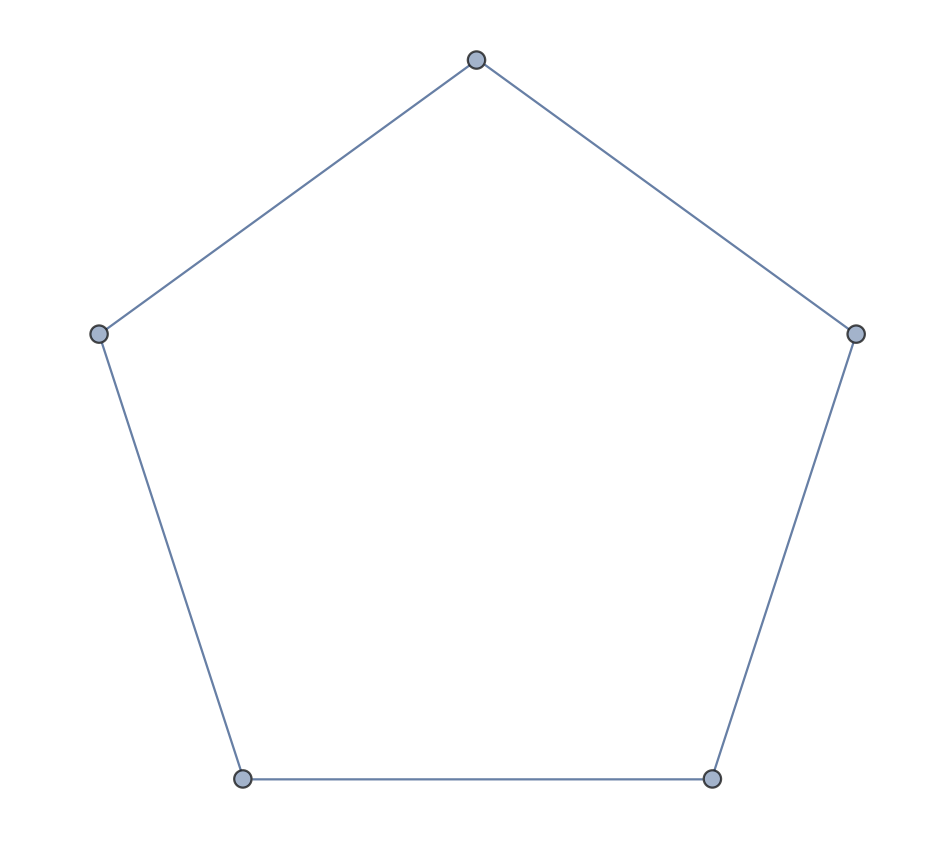
\includegraphics[width=50mm]{./figures/chapter1/cycle} &   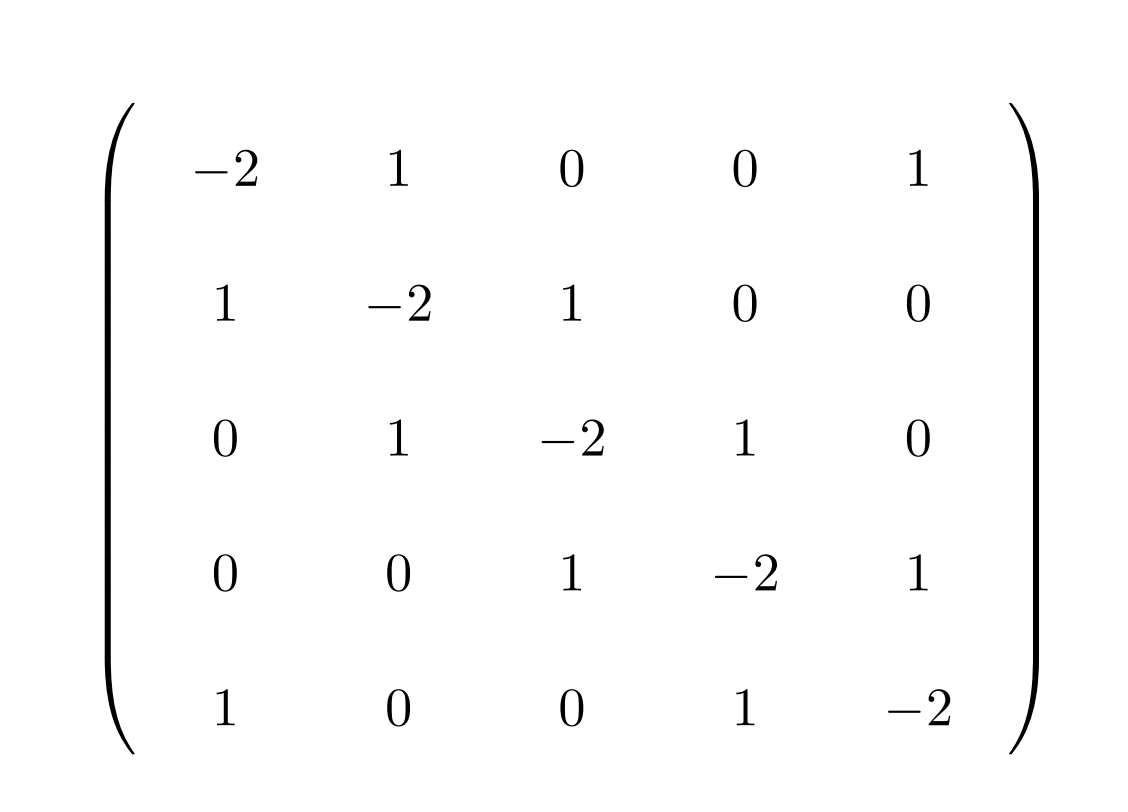
\includegraphics[width=50mm]{./figures/chapter1/cycleL} \\
          (a)  & (b) \\[6pt]
          \end{tabular}
          \caption[Pictorial representation of a cycle graph, and matricial representation for the Laplacian]{Pictorial representation of a cycle graph with 5 nodes (a), and the matricial representation for the Laplacian of Cy(5)}
        \end{figure}
    \vspace{-0.7cm}
    \subsection*{Complete Graph}
    \addcontentsline{toc}{subsection}{Complete Graph}
        A graph with N vertices is said to be complete if every node is adjacent to all the other N-1 nodes, thus representing a finite bidimensional structure. Its Laplacian matrix is given by:
        \begin{equation}
            L = (N-1)\sum_{j=1}^{N}\ket{j}\bra{j} - \sum_{k\neq j}\ket{j}\bra{k}
        \end{equation}
        A pictorial representation of a complete graph is given in figure. We will refere to this kind of graph with $C(N)$.
        \begin{figure}[hb]
          \centering
          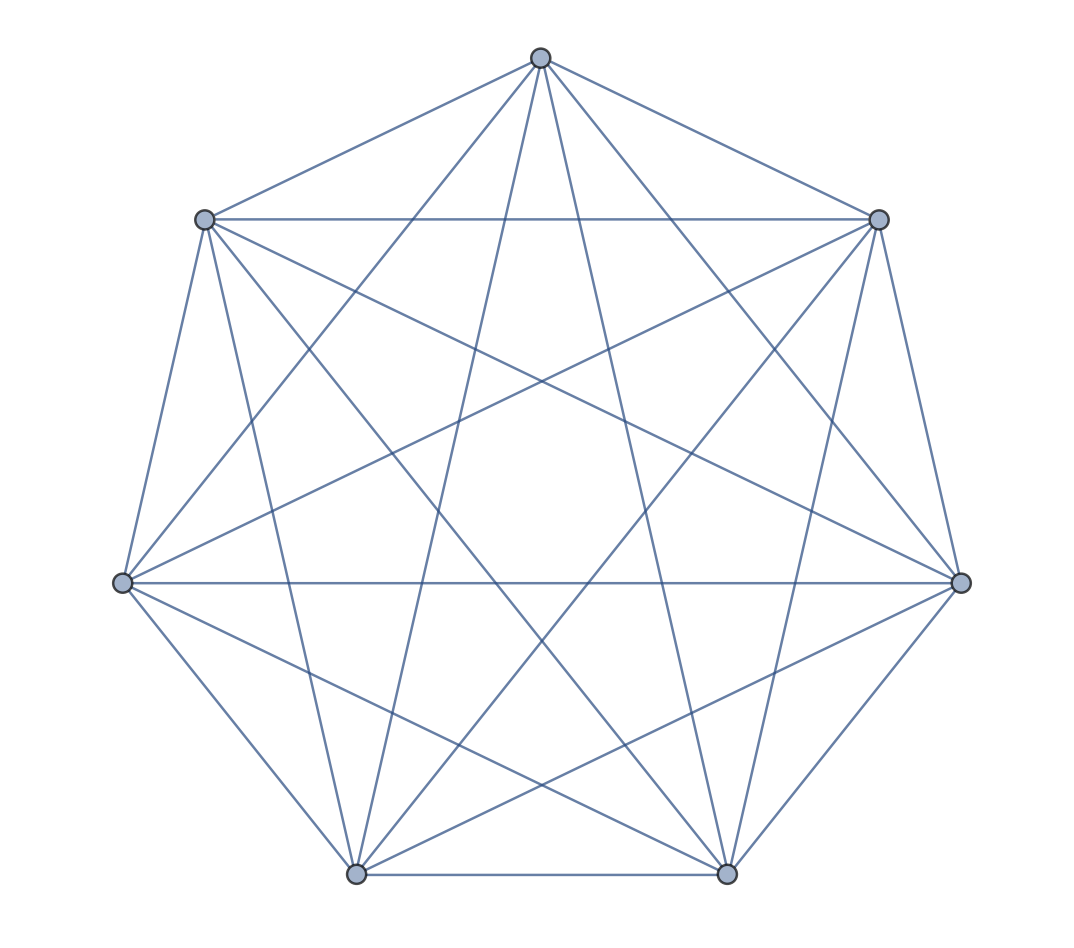
\includegraphics[width=50mm]{./figures/chapter1/complete}
          \caption[Pictorial representation of a complete graph]{Pictorial representation of a complete graph with N=7}
        \end{figure}

\section{Quantum Walks}
The continous time quantum walk (CTQW) is the direct analougue of the classical continous time random walk (CTRW). We begin by considering the classical one, expanding later on the quantum mechanical counterpart. \nocite{Mulken2011} \\
Let $j$ be a note of a graph $G$ and the initial node, such date the initial state of the system is $\ket{j}$. Then, we denote the transition probability of the walker to go from node j to a node k in a time t with $p_{k,j}(t)$. The state after time $t$ is given by $\ket{j;t}$, such that the overlap with node $k$ is $\braket{k|j;t}=p_{j,k}(t)$. \\
The dynamics resulting in the state $\ket{j;t}$ follows from transition rates per unit time between two nodes. In particular these transition rates are the components of the so-called \textit{transfer matrix} $T$, namely $T_{ij}= \bra{k}T\ket{j}$ . If we assume a Markovian process, the following master equation defines the CTRW evolution:
\begin{equation}
  \frac{d}{dt}p_{k,j}(t) = \sum_{l}T_{kl}p_{l,j}(t)
  \label{rw_master}
\end{equation}
In the simplest case, where the transitions rates for all edges are equal, the transfer matrix is closely related to the Laplacian matrix through :
\begin{equation}
  T = -\gamma L
\end{equation}
where $\gamma$ is the transition rate. The solution of \cref{rw_master}, along with the normalization constrains $\sum_{k=1}^{N}p_{k,j}(t) = 1 \hspace{3pt} \forall t$, is given by
\begin{equation}
  p_{ij}(t)= \braket{k|e^{Tt}|j} = \braket{k|e^{-\gamma At}|j}
\end{equation}
Turning to quantum mechanics the evolution of any physical system obeys the Schroedinger equation, and QWs represent no exception. The dynamics of the CTQW is governed by a specific Hamiltonian $H$, such that the Schroedinger equation for the transition \textit{amplitudes} $\alpha_{i,j}(t)$ is given by
\begin{equation}
  \frac{d}{dt}\alpha_{i,j}(t) = -i \sum_{l}H_{k,l}\alpha_{l,j}(t)
\end{equation}
where $H$ is the Hamiltonian of the systemm, and for semplicity we assume $\hbar = 1$. The formal solution of such differential equation is similarly to the CTRW given by
\begin{equation}
  \alpha_{l,j}(t) = \braket{k|e^{-iHt}|j}
  \label{qw_master}
\end{equation}
where $e^{-iHt}$ is the quantum mechanical time-evolution operator. We immediately notice the similar structure of equations (\ref{rw_master}) and (\ref{qw_master}), with the only difference apart from the imaginary unit  that the first is a differential equation for transition probabilities while the latter allows to compute transition amplitudes. The similarity is further pushed bu Farhi and Gutmann in 1998 \cite{Childs2001}, when they proposed to identify the Hamiltonian $H$ of the system with the negative of the classical transfer matrix $T$, which as we've seen previously is the Laplacian of the graph \footnote{Please note that in this particular scenario the transition amplitude $\gamma$ is set to one.}:
\begin{equation}
  H = -T = L
\end{equation}
Therefore the Laplacian matrix completely determines the evolution of the quantum system as well as the classical scenario.



\section{Grover's Quantum Search}
\red{This section should include the standard Grover's Quantum Search to give the contex for the quantum walk approach.}

\section{Spatial Search by Quantum Walk}
\purple{Spatial Search by Quantum Walk}{A. Childs, J. Goldstone}{quant-ph/0306054v2}\\
We now address the quantum search problem firstly formulated as Grover's algorithm and then extending it to the search on a graph using quantum walks. \\
To approach the Grover problem with quantum walk it's necessary to modify the hamiltonian such that the vertex $|w\rangle$, i.e. the target, is somewhat special. Following Grover's oracle an oracle hamiltonian $H_w$ is introduced

\begin{equation}
  H_w = -|w\rangle\langle w|
\end{equation}

which in particular has energy zero for all but the vertex $|w\rangle$ for which it has enenergy $-1$. Therefore the Grover problem, i.e. quantum search, becomes finding the ground state of such hamiltonian. To do so we consider the time-independent hamiltonian of the form
\begin{equation}
  H = -\gamma L + H_w = -\gamma L -|w\rangle\langle w|
\end{equation}
where L is the laplacian of the graph, which contains the information of the dynamics over that particular graph topology. The evolution of the quantum walk is therefore governed by this hamiltonian.\\

The quantum search routine works as follow:
\begin{itemize}
  \item we consider the superposition of all possible states, namely
  \begin{equation}
    |s\rangle = \frac{1}{\sqrt{N}}\sum_j|j\rangle
  \end{equation}

  \item we find the evolved state using the hamiltonian for a time T $H$
  \begin{equation}
  |\psi(T)\rangle = U(T)|s\rangle  = \mbox{exp}\Big\{-\frac{i}{\hbar}HT\big\}|s\rangle
  \end{equation}
  (Note that this evolution is valid only for time-independent hamiltonians.)

  \item we then measure the state onto the target $|w\rangle$ and find the corrisponding probability
  \begin{equation}
    p = |\langle w|\psi(T)\rangle|^2
  \end{equation}

\end{itemize}

The objective is to find the optimal value of $\gamma$ so that the probability of the system of finding itself in $|w\rangle$ is as close as possible to 1 for the smallest T.

\subsection{Search on Complete Graph}
We now look at the search on a complete graph. This case is particularly interesting since it can be solved analitically\\
\red{to be continued}

\section{Adiabatic Theorem}
\purple{Quantum Computation by Adiabatic Evolution}{E. Farhi, J. Goldstone, S. Gutmann, M. Sipser}{quant-ph/0001106}\\


A quantum system evolves according to the Schroedinger equation
\begin{equation}
    i\frac{d}{dt}|\psi(t)\rangle = H(t)|\psi(t)\rangle
\end{equation}
and defining the instantaneous eigenstates and eigenvalues of H(t) by
\begin{equation}
    H(t)|l;t\rangle = E_l(t)|l;t\rangle
\end{equation}
such that $E_0(t) \geq E_1(t) \geq ... \geq E_{N-1}(t)$. \\
The adiabatic theorem states that if the gap between the two lowest energy levels, $E_{1}(t) - E_{0}(t) > 0$, is stritcly greater than zero then for $T\rightarrow \infty$ the probability of being in the ground state is equal to one, namely
\begin{equation}
    \lim_{T \to \infty} |\langle l=0;t = T | \psi(T)\rangle| = 1
\end{equation}
This means that if the system is chosen to evolve at a slow enough rate, the instantaneous hamiltonian will remain in the ground state throught the evolution. It is useful to consider a smooth one-parameter hamiltonian $H(s)$ such that $s=t/T$, with $t \in [0,T]$ so that $s \in [0,1]$.
Let's now define the energy minimum gap by
\begin{equation}
    g_{min} = \min_{0 \leq s \leq 1} (E_1(s)-E_0(s))
\end{equation}
In addition we can find a time lower bound $T^*$ such that for $T\gg T^{*}$ the probability is arbitrarily close to 1, in detail
\begin{equation}
    T \gg \frac{\varepsilon}{g^{2}_{min}}
\end{equation}
where
\begin{equation}
    \varepsilon = \max_{0 \leq s \leq 1} \Big| \Big\langle l=1;s\Big| \frac{dH(s)}{dt} \Big| l=0;s\Big\rangle\Big|
\end{equation}

\subsection{Computation by Adiabatic Evolution}
Let's now discuss how to take advantage of the adiabatic theorem introducting the usual way in which the adiabatic evolution is implemented. It is often presented a problem hamiltonian $H_P$ whose ground state is not so straight forward to find; on the other hand we can prepare the system in abeginning hamiltonian $H_B$ whose ground state is known. The problem hamiltonian encodes the solution of the problem, while the beginning hamiltonian is a tool for easily preparing the state to be evolved. The adiabatic implementation then consists, assuming that the ground state of $H_P$ is unique, in having a time dependent hamiltonian $H(s)$ such that
\begin{equation}
    H(s) = (1-s)H_B + s H_P
\end{equation}
In this way we can prepare for $s=0$ the system in $H_B$ and let it evolve so that for $s=1$ it reaches $H_P$. Thanks to the adiabatic theorem, if it's made to evolve sufficiently slowly we will find ourself in the ground state of the problem hamiltonian, which is exactly the solution.

\section{Impossibility of Adiabatic Quantum Walks}
\cite{Wong2016}
